\section{Experiments}
\label{sec-quant}
\begin{figure}
  \centering
  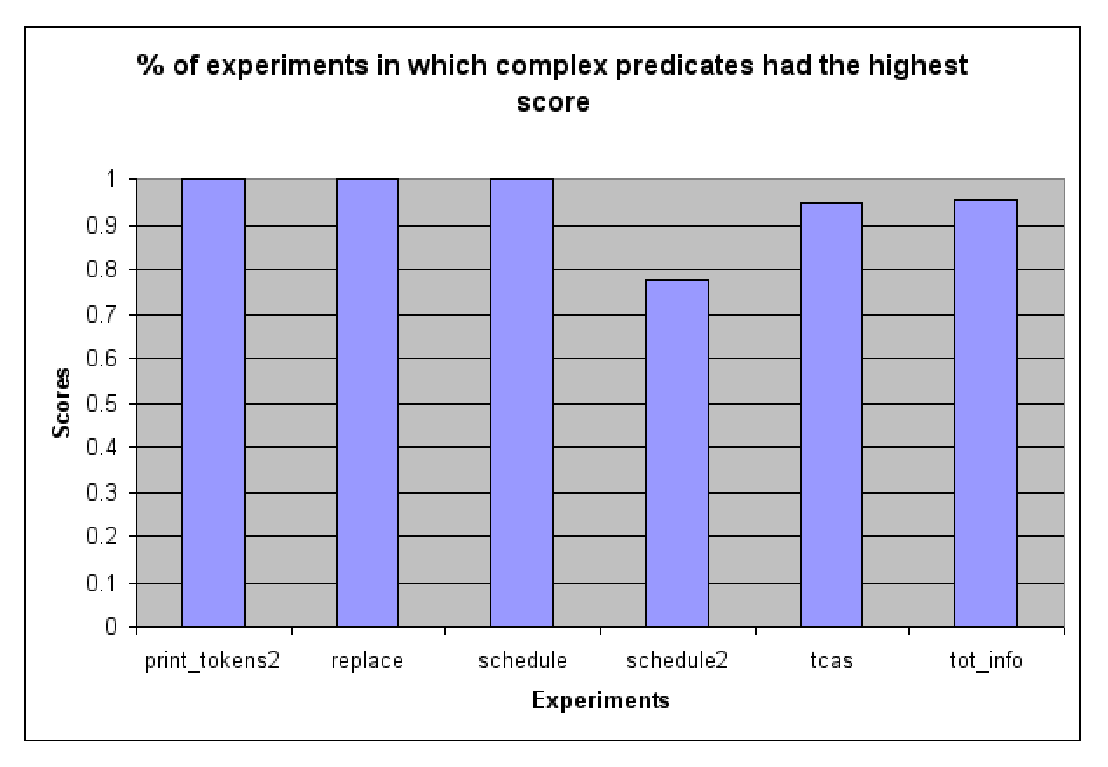
\includegraphics[width=\columnwidth]{charts/top-pred}  
  \caption{Complex predicates having the highest score}
  \label{fig-top-pred}
\end{figure}

\begin{figure}
  \centering
  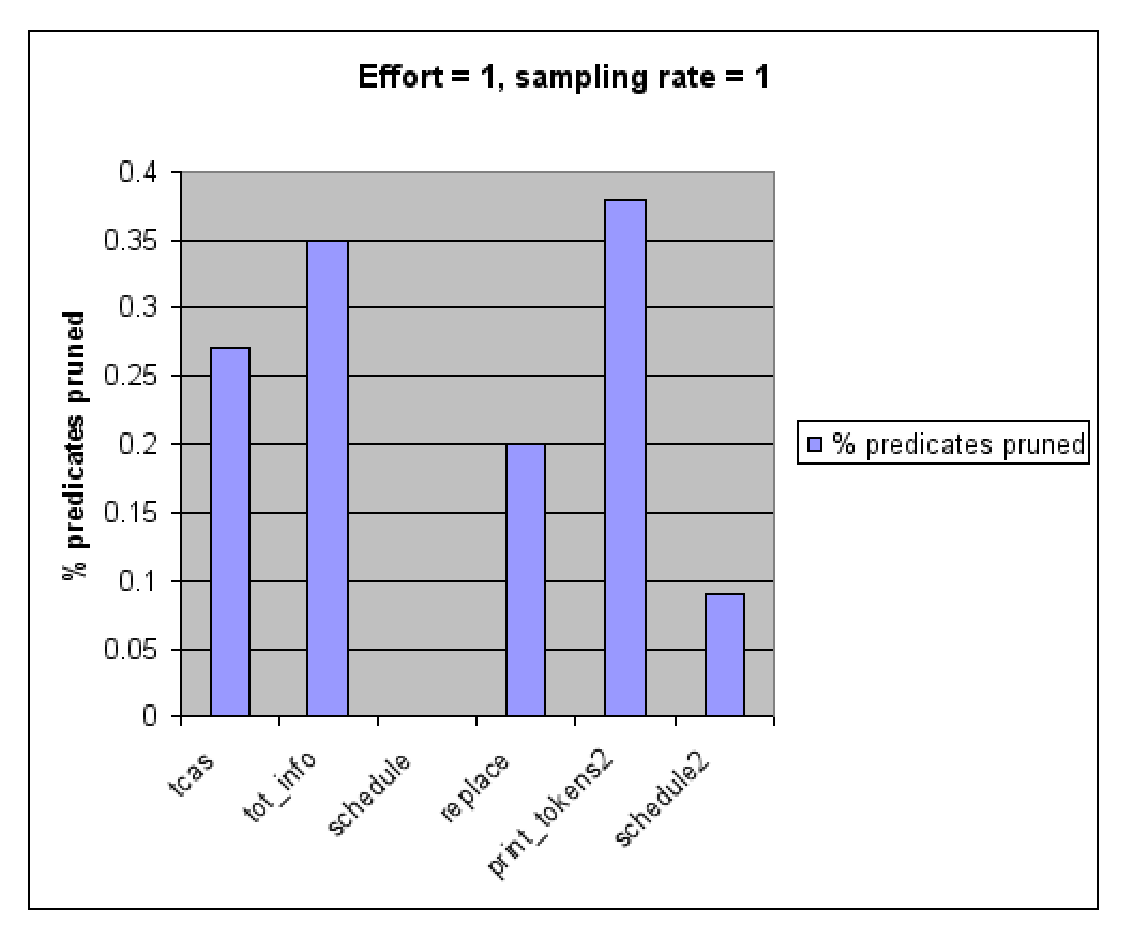
\includegraphics[width=\columnwidth]{charts/pruning}
  \caption{Improvement from pruning}
  \label{fig-pruning}
\end{figure}

\begin{figure}
  \centering
  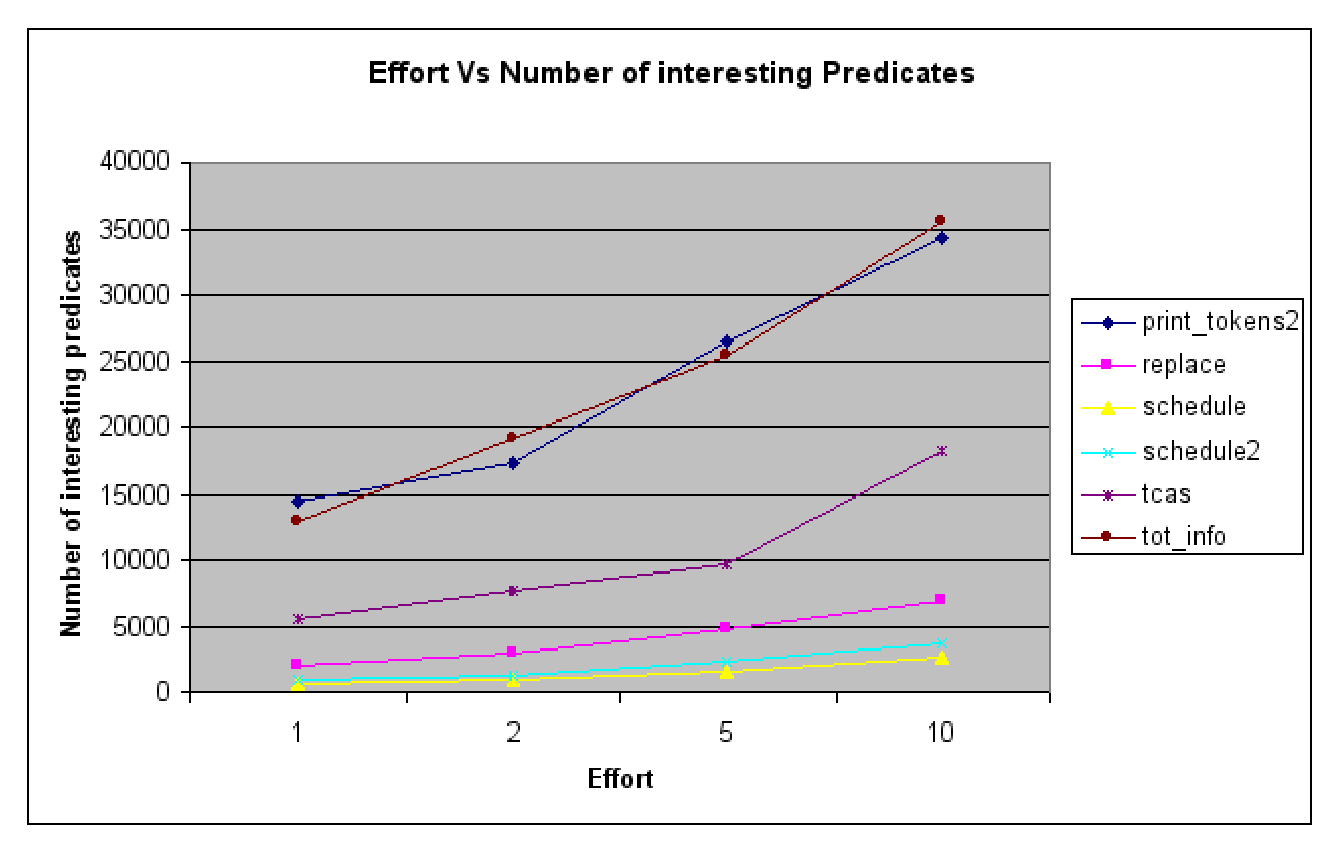
\includegraphics[width=\columnwidth]{charts/effort}
  \caption{Variation of number of interesting predicates with $effort$}
  \label{fig-effort}
\end{figure}

\begin{figure*}
  \centering
  $\begin{array}{cc}
    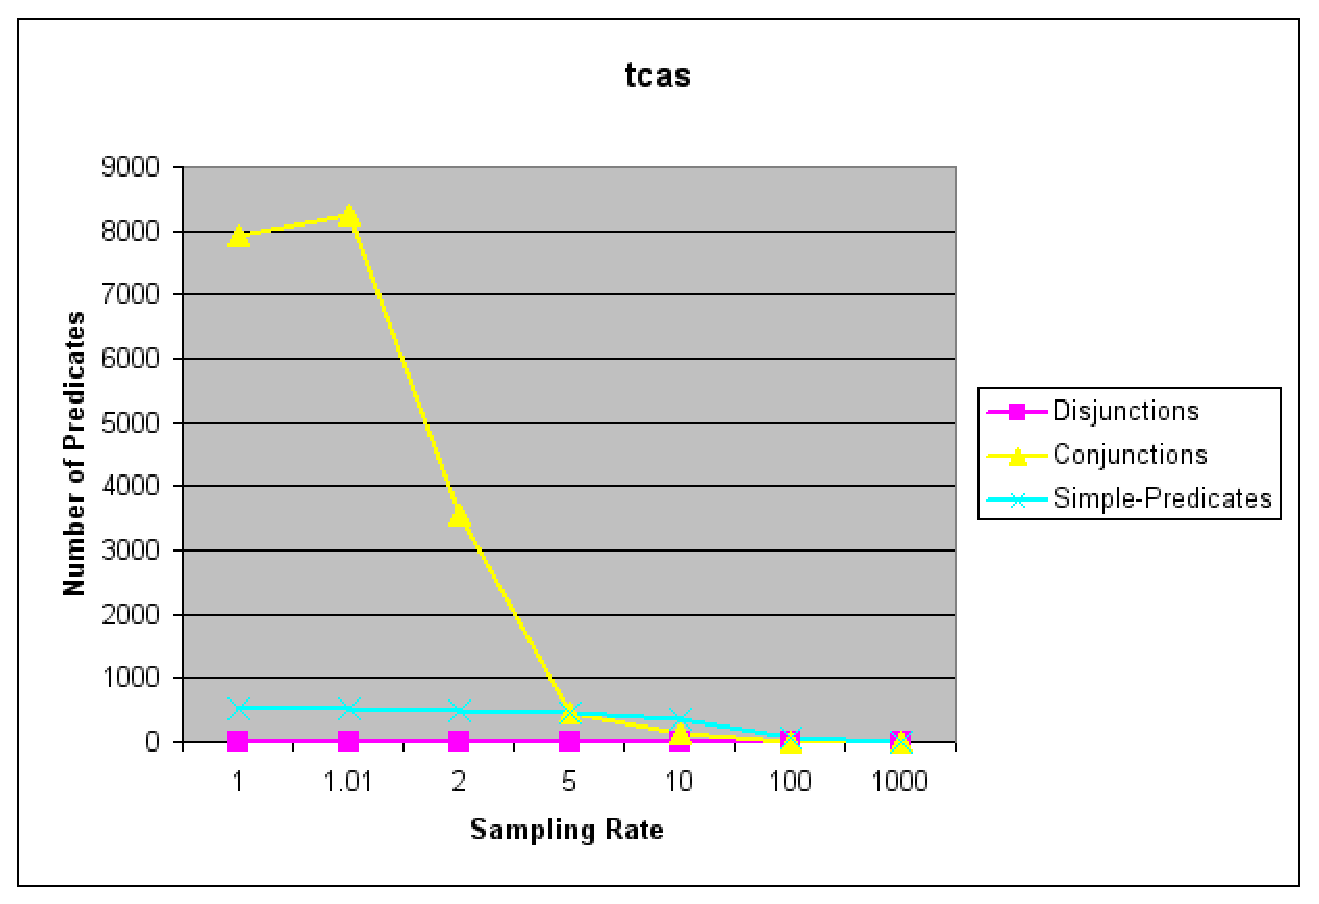
\includegraphics[width=\columnwidth]{charts/tcas} & 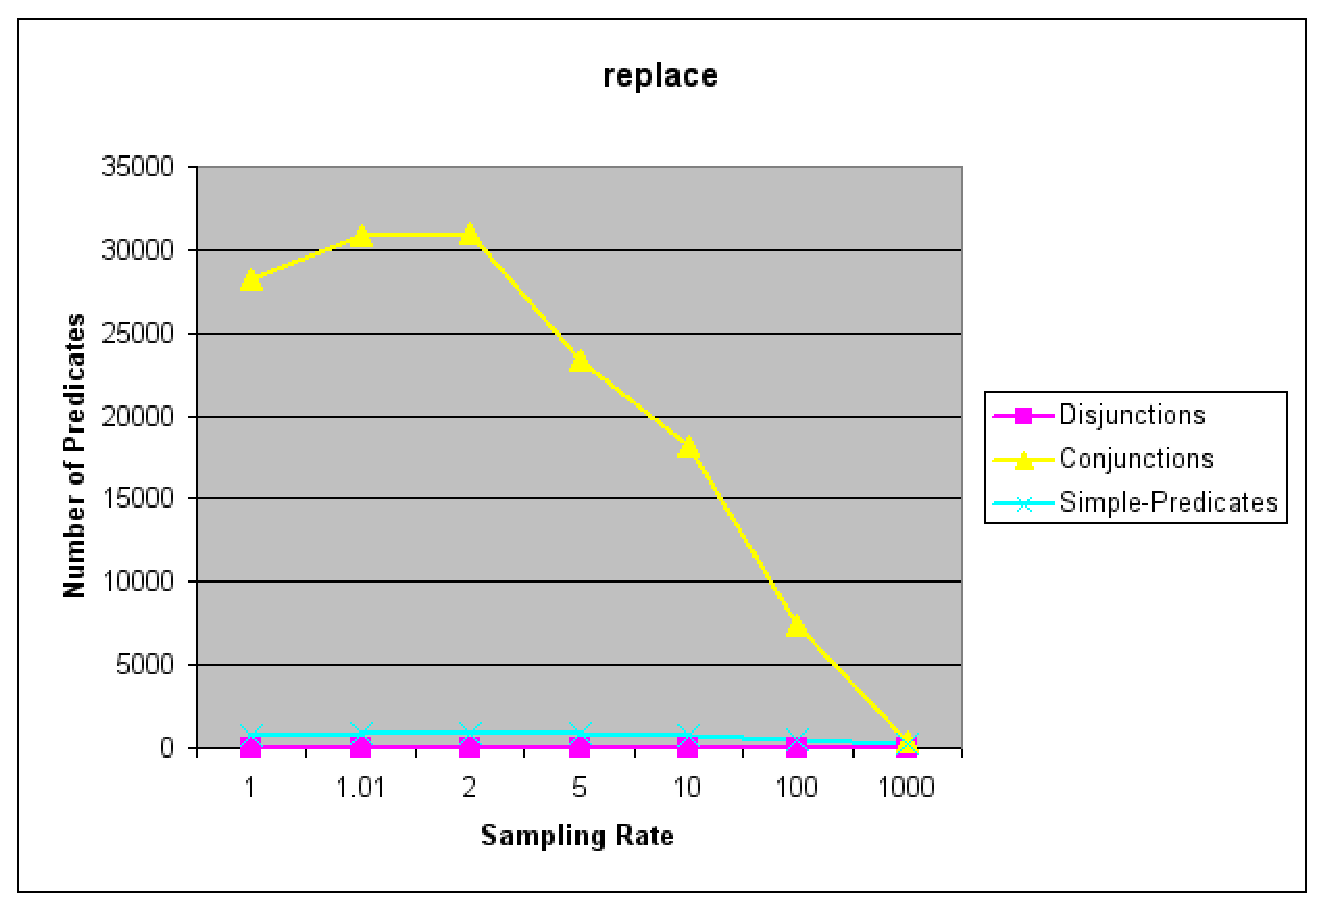
\includegraphics[width=\columnwidth]{charts/replace} \\
    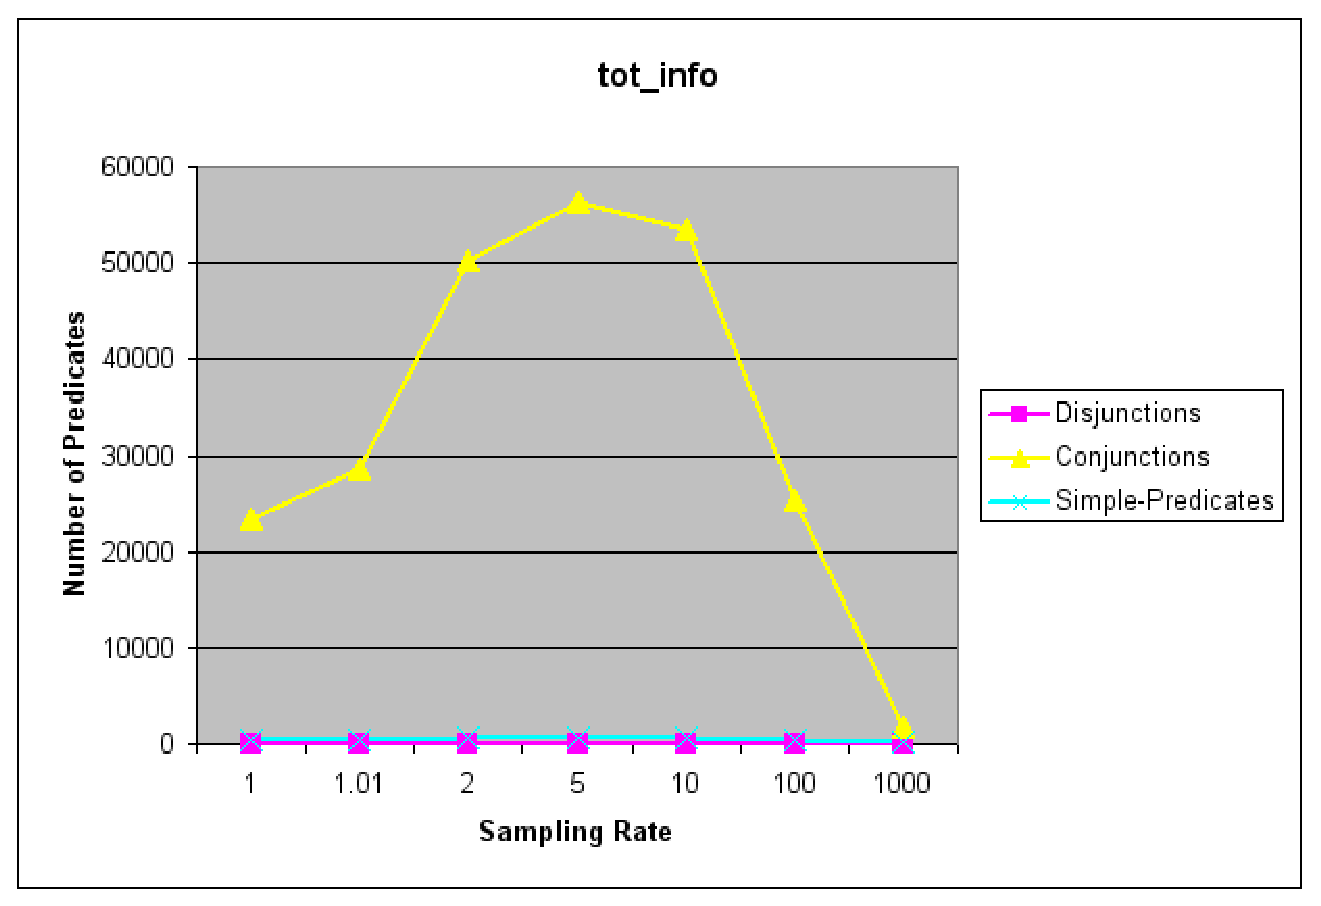
\includegraphics[width=\columnwidth]{charts/tot_info} & 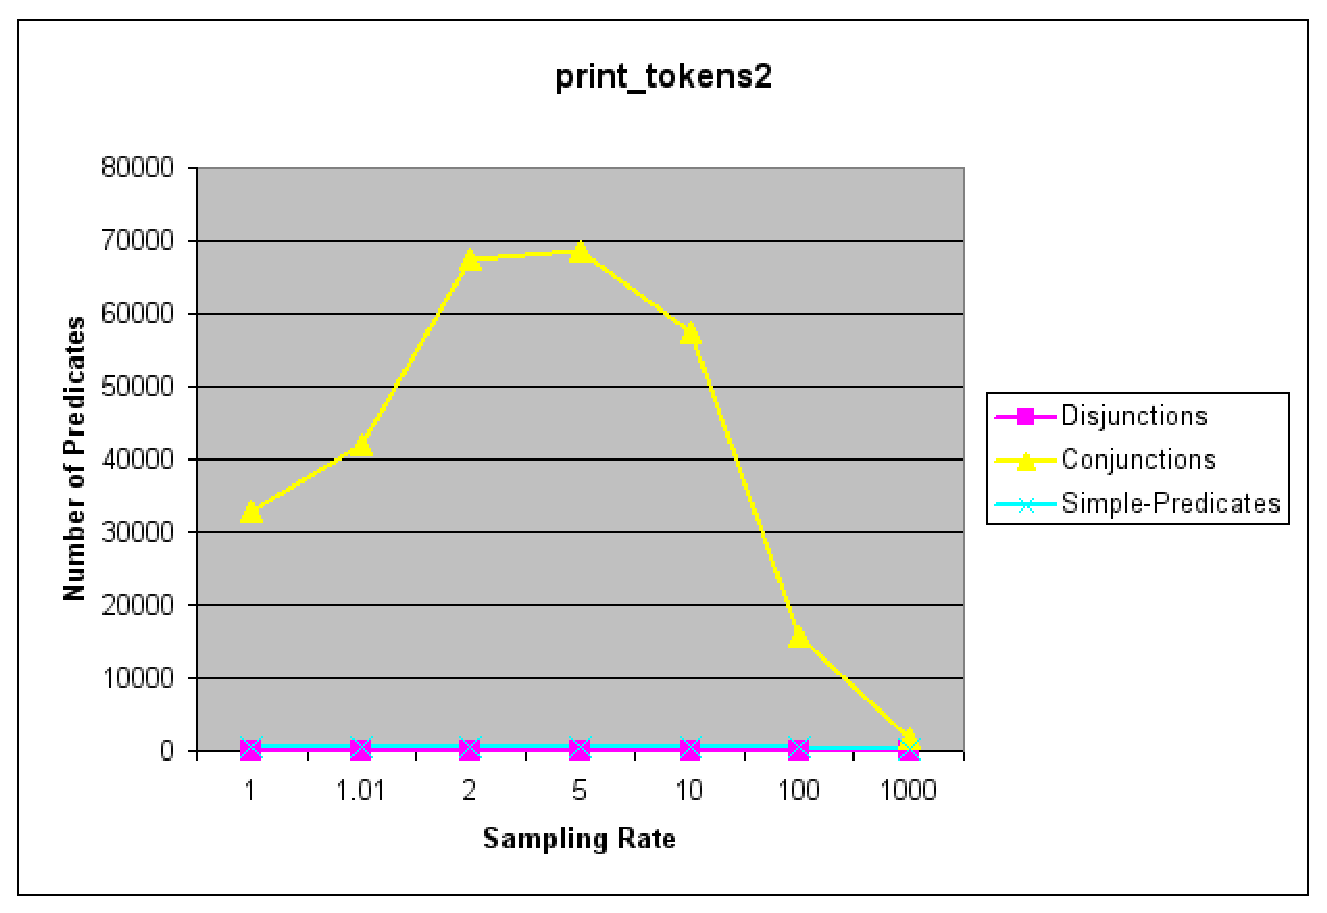
\includegraphics[width=\columnwidth]{charts/print_tokens2} \\
    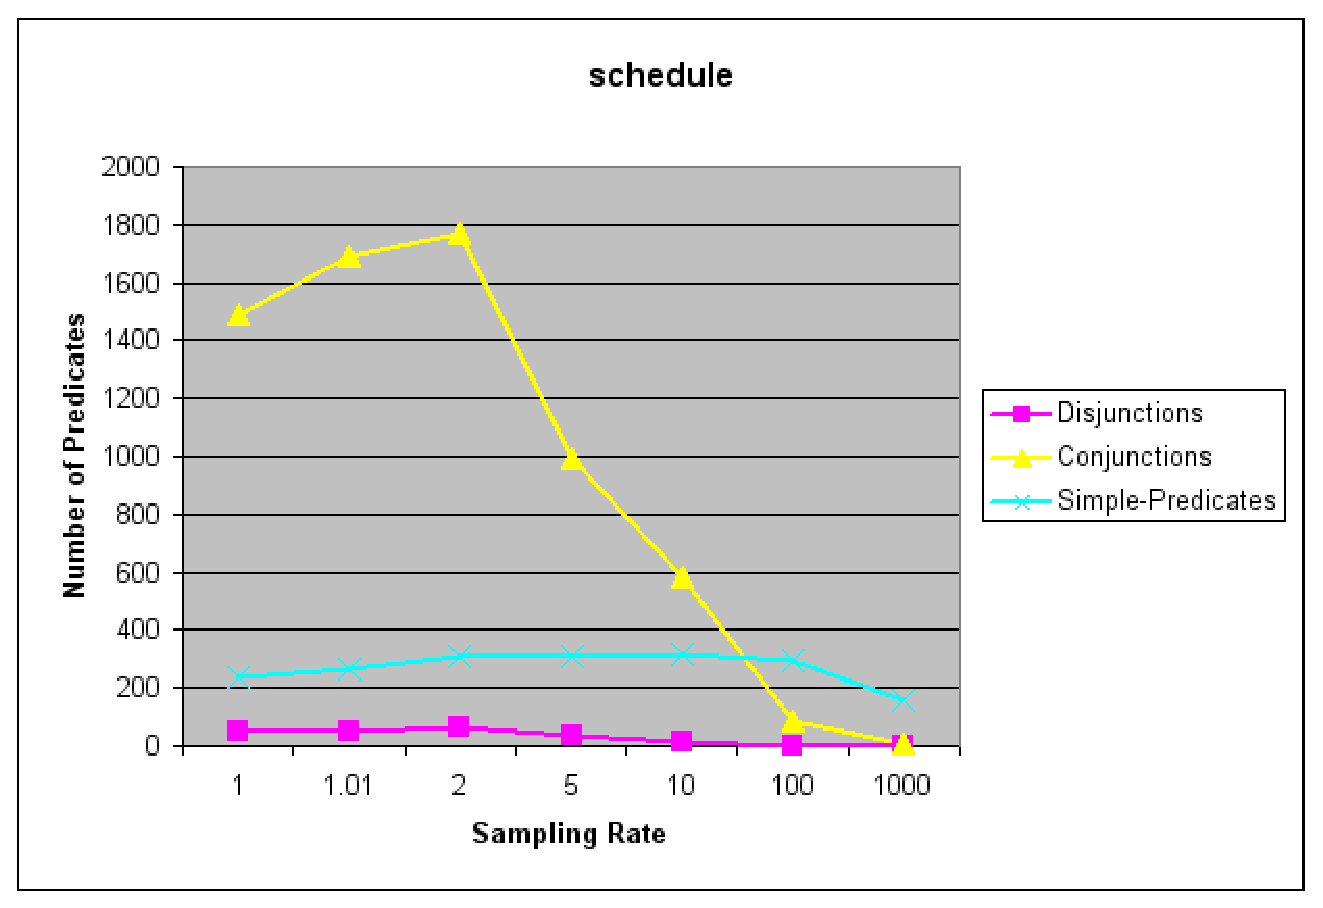
\includegraphics[width=\columnwidth]{charts/schedule} & 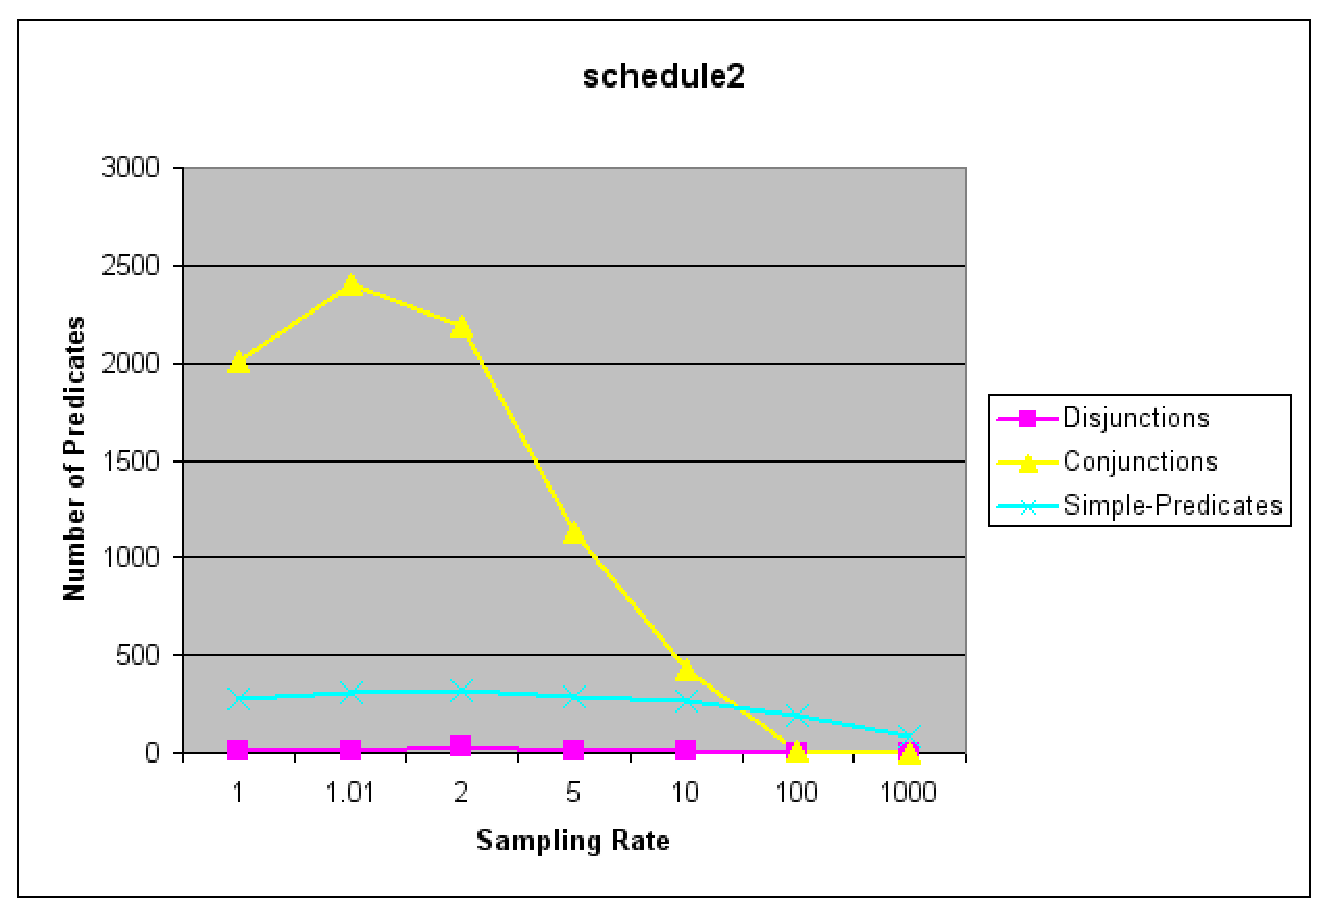
\includegraphics[width=\columnwidth]{charts/schedule2} \\
  \end{array}$
  \caption{Sampling Rate vs. Number of Predicates}
  \label{fig-sampling}
\end{figure*}

This section presents quantitative data about the ideas presented in previous sections.  This data was collected using the Siemens test suite~\cite{257766}.  There are two configurable parameters for the experiments: the rate of sampling and $effort$ (described in ~\autoref{sec-metrics}).  Unless specified, the default sampling rate is 1 (i.e. complete data collection) and the default $effort$ is 5\% (only predicates that are reachable from each other by exploring less than 5\% of the program are considered).

\subsection{Top Scoring Predicates}
~\autoref{fig-top-pred} plots the percentage of variants within each program for which a complex predicate had the highest score among all predicates.  The value is 100\% for \texttt{print\_tokens2, replace} and \texttt{schedule} and is close to 100\% for the other programs.  The results shown in ~\autoref{fig-top-pred} combined with the case studies in ~\autoref{sec-qual} demonstrates the usefulness of complex predicates.

\subsection{Improvement from Pruning}
~\autoref{fig-pruning} shows the percentage of complex predicates that are pruned by the optimizations discussed in ~\autoref{sec-pruning} and the metrics in ~\autoref{sec-metrics}.  For each program, the y-axis shows the contribution of the two kinds of pruning.  On average, the usefulness metrics prune 54\% of complex predicates and the optimizations in ~\autoref{sec-pruning} prune 15\% of complex predicates.  Only 31\% of the complex predicates are actually computed.

\subsection{Effect of the $Effort$ Parameter}
~\autoref{fig-effort} has one curve for each program showing how the number of interesting predicates (~\autoref{dfn3}) varies at four different values - 1, 2, 5, 10 for $effort$.  As expected, as $effort$ increases more predicates are evaluated and so more interesting predicates are found.  This experiment serves as a sanity check for the implementation.

\subsection{Effect of Sampling Rate}
\label{sec-sampling}
The dependence between sampling rate and the number of interesting predicates (both complex and simple) is plotted in ~\autoref{fig-sampling}.  ~\autoref{fig-sampling} has one chart per program with sampling rates in the $x-$axis and the average number of interesting conjunctions, disjunctions and simple predicates in the $y-$axis.  The number of interesting disjunctions is always very low (order of tens) compared to interesting conjunctions.  So the plot for interesting complex predicates closely follows the plot for conjunctions.  At sampling rates higher than 10, there is a sharp drop in the number of interesting conjunctions.  This is because with a sampling rate of $N$, the chance of observing a complex predicate is close $\frac{1}{N^2}$ {\footnote{it is not equal to $\frac{1}{N^2}$ because of short circuiting boolean operations}}.  Despite the sharp drop, the number of interesting conjunctions is still comparable to the number of interesting simple predicates.  This shows that sparse random sampling is not a significant detriment in finding interesting complex predicates.

A puzzling trend in ~\autoref{fig-sampling} is that interesting conjunctions increases for a brief interval before dropping off.  This trend is consistent across all programs.  This can be due to two reasons:
\begin{enumerate}
\item Consider the $Increase$ score (Eqn ~\ref{eqn1}).  Sampling may be reducing the number of $observed$ runs in which a conjunction was true without affecting the $true$ runs.  This could happen because we do not collect sampled data directly but use scripts to down sample a data set collected with no sampling.  Because of binarization of counts, down sampling of a count from 100 to 99 does not affect the score whereas down sampling from 1 to 0 affects the score. 
\item The script that does down sampling uses the standard pseudo random number generator.  Usually for experiments that use such random data, the values are averaged over multiple trials to get a confident estimate of the results.  We weren't able to conduct multiple trials because of time constraints.
\end{enumerate}
